%% LyX 2.2.2 created this file.  For more info, see http://www.lyx.org/.
%% Do not edit unless you really know what you are doing.
\documentclass[english]{article}
\usepackage[T1]{fontenc}
\usepackage[latin9]{inputenc}
\usepackage{float}
\usepackage{graphicx}

\makeatletter

%%%%%%%%%%%%%%%%%%%%%%%%%%%%%% LyX specific LaTeX commands.
%% Because html converters don't know tabularnewline
\providecommand{\tabularnewline}{\\}

\makeatother

\usepackage{babel}
\begin{document}

\part{ELECTRONICA III - EJERCICIO 1}

\section{Implementaci�n de Compuertas Not con Transistores}

En esta primer parte del art�culo se propondr� a realizar una compuerta
b�sica como es la inversora, o tambi�n llamada ``NOT'', con transistores.
Los dise�os que se muestran a continuaci�n son cuatro: dos variantes
con transistores bjt y otras dos con transistores mosfet.

\begin{figure}[H]
\begin{centering}
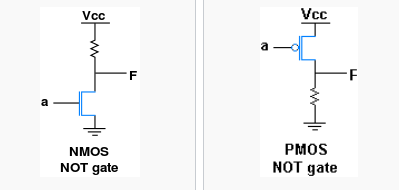
\includegraphics[scale=0.4]{mosNOT.PNG}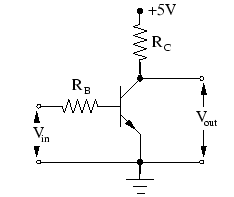
\includegraphics[scale=0.4]{npnNOT.PNG}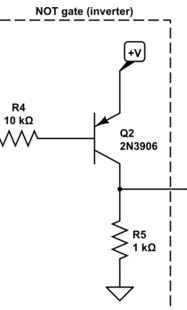
\includegraphics[scale=0.4]{pnpNOT.PNG}
\par\end{centering}
\caption{Dise�o de NOT con Transistores}

\end{figure}

Como se muestra en las imagenes, dentro de la variante de los mosfet
se utiliz� el transistor NMOS y el PMOS. En cuanto a los transistores
bipolares, se propuso un modelo con NPN y otro con PNP.

Una vez materializados estos dise�os, se procedi� a medir algunos
par�metros que caracterizan a la compuerta l�gica. Vale aclarar que
las mediciones se realizaron solo para las compuertas con transistores
bipolares.

A continuaci�n se muestran los resultados de las mediciones sin carga:

\begin{table}
\begin{tabular}{|c|c|c|}
\hline 
sin carga & NPN & PNP\tabularnewline
\hline 
\hline 
High-level input voltage (V) & 1 & 4,5\tabularnewline
\hline 
Low-level input voltage (V) & 0,400 & 4,2\tabularnewline
\hline 
High-level output (V) & 4,930 & 4,93\tabularnewline
\hline 
Low-level output (V) & 0,075 & 0,05\tabularnewline
\hline 
High Level Noise Margin (V) & 3,930 & 0,43\tabularnewline
\hline 
\end{tabular}%
\begin{tabular}{|c|c|c|}
\hline 
sin carga & NPN & PNP\tabularnewline
\hline 
\hline 
Low Level Noise Margin (V) & 0,325 & 4,150\tabularnewline
\hline 
Propagation delay High-Low  & 2,295 us & 140 ns\tabularnewline
\hline 
Propagation delay Low-High & 130 ns & 930 ns\tabularnewline
\hline 
Transition tiem High-Low & 1,470 us & 89 ns\tabularnewline
\hline 
Transition time Low-High & 98,500 us & 1,400 us\tabularnewline
\hline 
\end{tabular}

\caption{Mediciones - Par�metros Compuerta NOT - sin carga}
\end{table}

Luego se realizaron las mismas mediciones con una carga capacitiva:

\begin{table}
\begin{tabular}{|c|c|c|}
\hline 
con carga & NPN & PNP\tabularnewline
\hline 
\hline 
High-level input voltage (V) & 0,9 & 4,5\tabularnewline
\hline 
Low-level input voltage (V) & 0,5 & 4,2\tabularnewline
\hline 
High-level output (V) & 4,89 & 4,92\tabularnewline
\hline 
Low-level output (V) & 0,074 & 0,06\tabularnewline
\hline 
High Level Noise Margin (V) & 3,99 & 0,42\tabularnewline
\hline 
\end{tabular}%
\begin{tabular}{|c|c|c|}
\hline 
con carga & NPN & PNP\tabularnewline
\hline 
\hline 
Low Level Noise Margin (V) & 0,0426 & 4,14\tabularnewline
\hline 
Propagation delay High-Low & 11,200 us & 165 ns\tabularnewline
\hline 
Propagation delay Low-High & 172,50 ns & 5,100 us\tabularnewline
\hline 
Transition tiem High-Low & 5,700 us & 164 ns\tabularnewline
\hline 
Transition time Low-High & 196 ns & 11,350 us\tabularnewline
\hline 
\end{tabular}

\caption{Mediciones - Par�metros Compuerta NOT - con carga}
\end{table}

Todas las mediciones se realizaron con Vcc igual a 5 Volts. En cuanto
a las mediciones de tiempo de propagaci�n y de transici�n, para estas
se utiliz� una excitaci�n de onda cuadrada de 1,92 KHz.
\end{document}
